\section{Power analysis}

% Slide 1: What is a Power Analysis Attack?
\begin{frame}
    \frametitle{What is a Power Analysis Attack?}

    \begin{alertblock}{}
        Switching 1 $\rightarrow$ 0 and 0 $\rightarrow$ 1 means providing or removing power to transistors.\newline
        A power analysis attack is a technique that exploits the relationship between a device's \textbf{power consumption} and the \textbf{data it processes}  or the \textbf{operations} performed.

        By carefully measuring power usage, an attacker can learn about the secret data being used
    \end{alertblock}

    
\end{frame}

\begin{frame}
    \frametitle{The Attack Setup}

        The setup for a power analysis attack is composed of:
        \begin{itemize}
            \item A \textbf{target device} that performs cryptography.
            \item A small \textbf{resistor} placed in the power line of the device.
            \item A digital \textbf{oscilloscope} to measure the tiny voltage changes across the resistor.
        \end{itemize}
        The oscilloscope captures a \textbf{power trace}: a graph of power usage over time.


    \begin{figure}
        \centering
        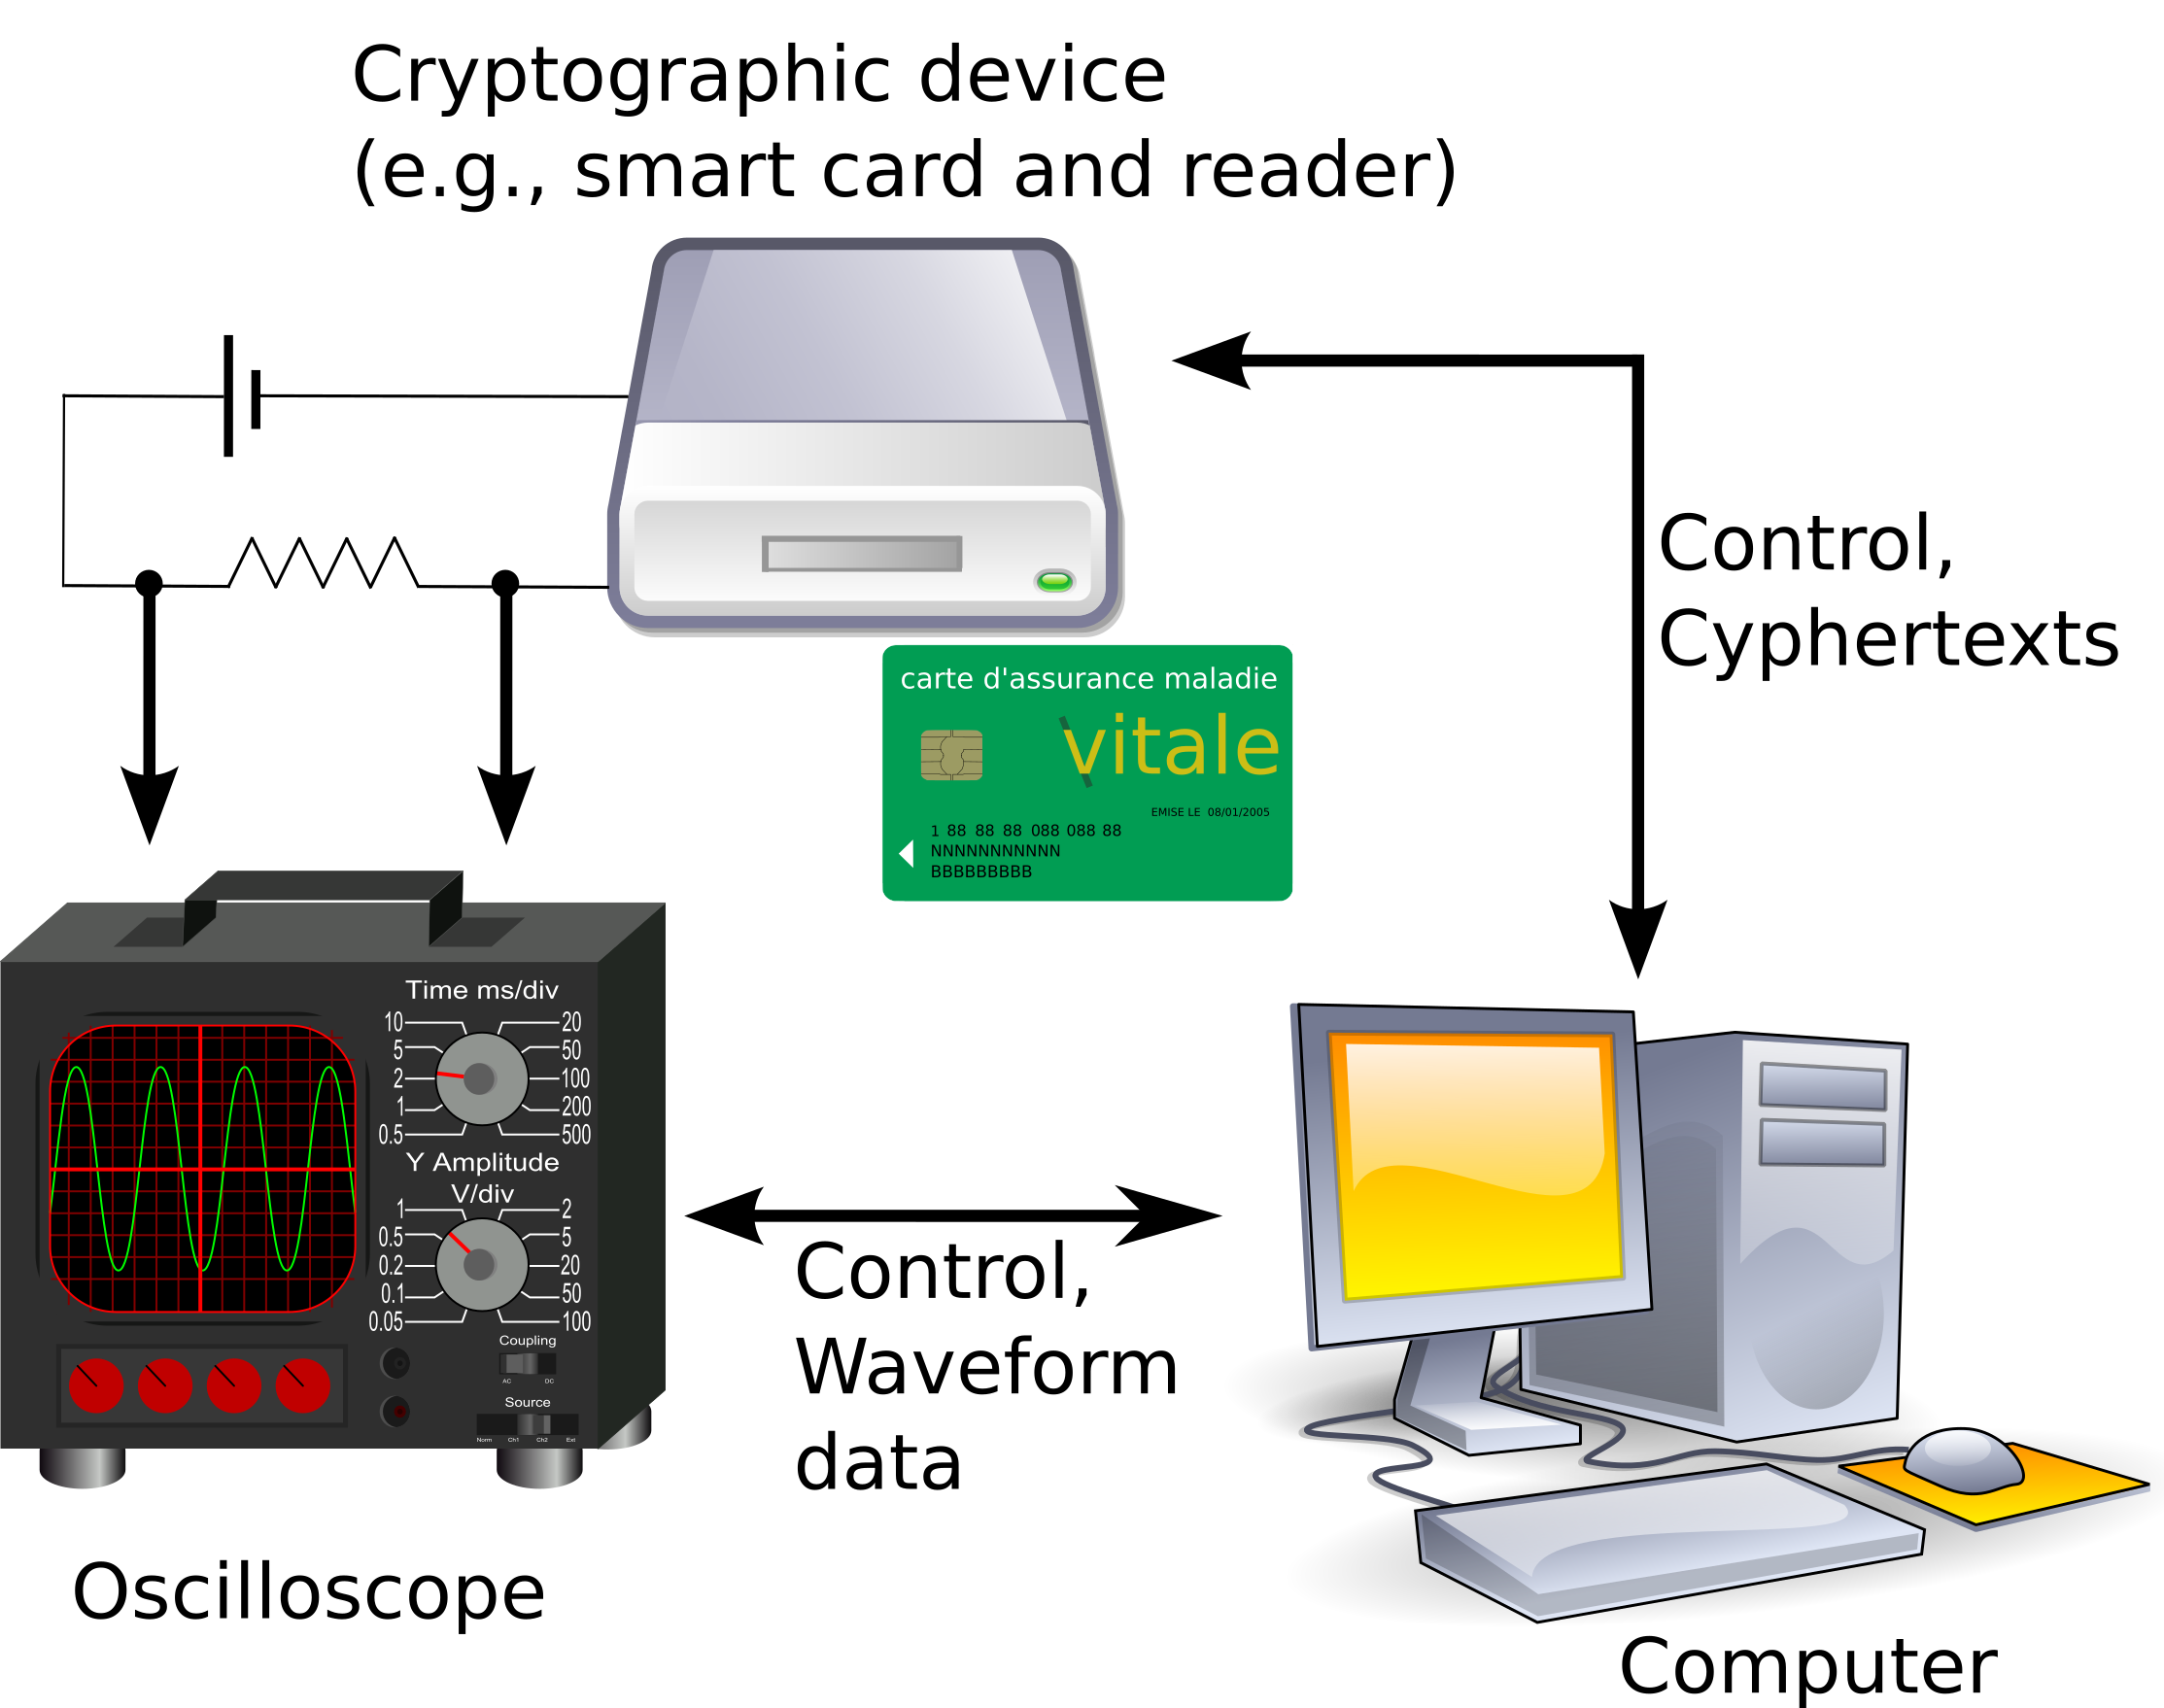
\includegraphics[width=0.45\textwidth]{main thing/Pictures/scheme2_oscilloscope.png}
       
    \end{figure}
\end{frame}

\begin{frame}
    \frametitle{Possible target devices}

    Electronic devices that perform cryptographic computations can be power analysis targets. This includes:
    \begin{itemize}
        \item Smart Cards and Security Tokens
        \item Embedded Microcontrollers (MCUs)
        \item Internet of Things (IoT) Devices
        \item Mobile Phones and Tablets
    \end{itemize}
    \begin{columns}[T] % The 'T' option aligns the columns at the top
        \begin{column}{0.40\textwidth}
            \centering
            
\includegraphics[width=\linewidth]{main thing/Pictures/smartcard.png}
        \end{column}
        
        \begin{column}{0.48\textwidth}
            \centering
            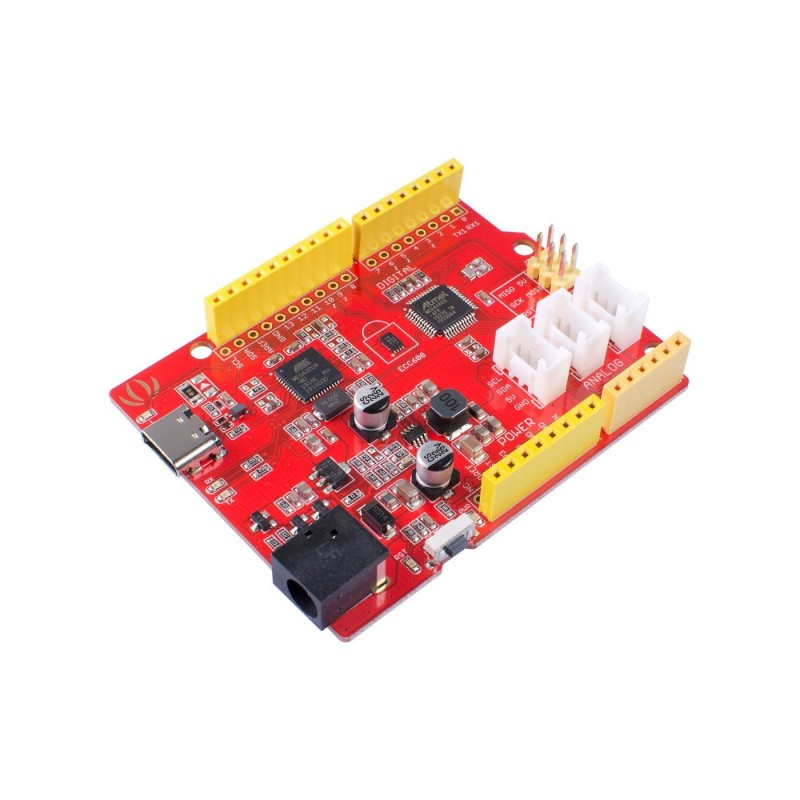
\includegraphics[width=\linewidth]{main thing/Pictures/mcu.jpg}
        \end{column}
    \end{columns}
\end{frame}

\begin{frame}
    \frametitle{The Goal of Power Analysis attacks}

    \begin{block}{Retrieving the Secret Key}
        The primary goal of most power analysis attacks is to recover secret \textbf{cryptographic keys}.
    \newline
        This is rarely done by attacking the full key at once. Instead, attackers target \textbf{intermediate values} that are processed during the cryptographic algorithm. By learning small pieces of the key one at a time, they can eventually reconstruct the entire secret.
    \end{block}
   
\end{frame}





\begin{frame}
    \frametitle{The Power Trace: A Measurement Vector}

    \begin{block}{Definition}
        A power trace is a discrete time-series vector representing the instantaneous power consumption of a cryptographic device during a specific operation.
        \begin{itemize}
            \item Each point in the trace corresponds to a power measurement at a discrete point in time, captured by a high-frequency sampling instrument like a digital oscilloscope.
            \item The trace represents the electrical activity of the device's components.
        \end{itemize}
    \end{block}

    \begin{figure}
        \centering
        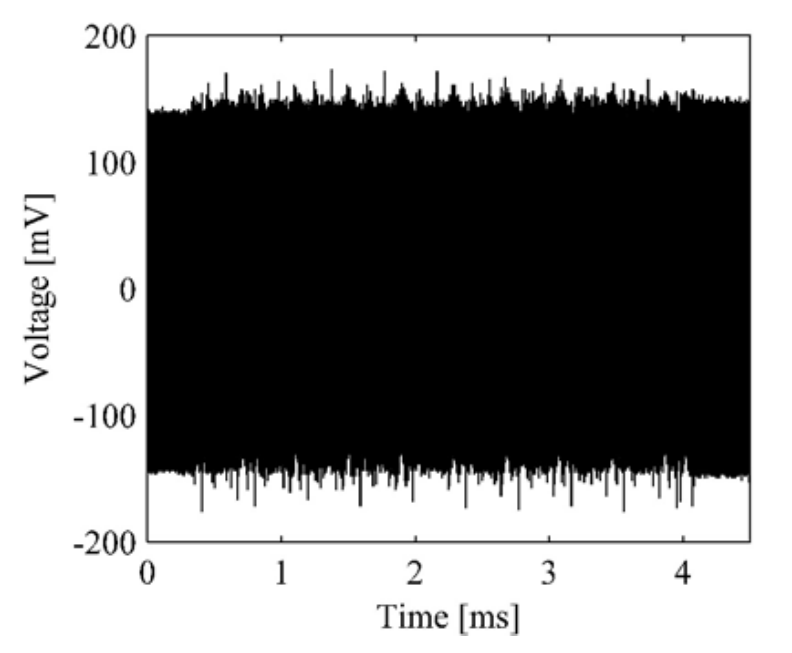
\includegraphics[width=0.35\linewidth]{main thing/Pictures/trace.png}
    \end{figure}
\end{frame}

\begin{frame}
    \frametitle{The Non-Deterministic Nature of Measurements}

    \begin{block}{The Problem of Measurement Variance}
        Repeated measurements of the same operation, using the \textbf{exact same inputs} (key and plaintext), will yield different power traces.\newline
        This variability is due to the presence of \textbf{noise}.
    \end{block}
    
    \begin{figure}
        \centering
        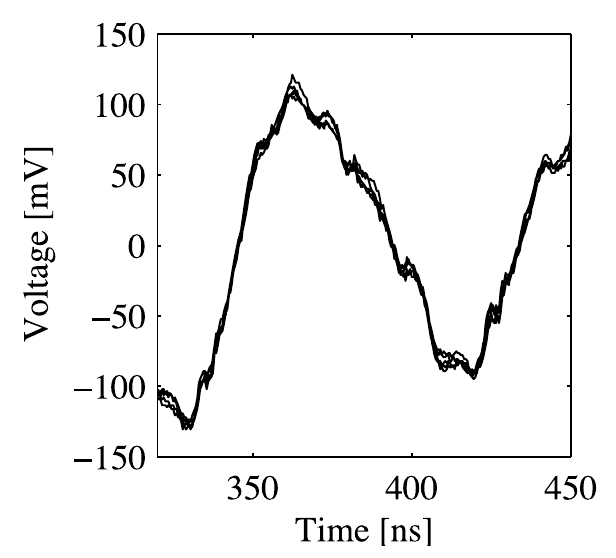
\includegraphics[width=0.4\linewidth]{main thing/Pictures/noise.png}
        \caption{Power traces are different (but look very similar) even processing the same input because of noise}
    \end{figure}
\end{frame}


\begin{frame}
    \frametitle{Noise Source 1: Electronic Noise}

    \begin{block}{The Stochastic Component}
        \textbf{Electronic Noise}, $P_{electronic\_noise}$, is originated by the physical properties of the electronic components and the measurement setup.\newline
        It has many sources:
        
        \begin{itemize}
            \item Power supply
            \item Clock generator
            \item Radiated emissions of neighboring components
        \end{itemize}
    \end{block}
    \begin{alertblock}{}
        The distribution of the electronic noise $P_{el.noise}$ is a normal distribution
        $$P_{el.noise} \sim \mathcal{N(0, \sigma)}$$
    \end{alertblock}
\end{frame}

\begin{frame}
    \frametitle{Noise Source 2: Switching Noise}

    \begin{block}{The Uncorrelated Component}
        \textbf{Switching Noise} is the variations of power traces that are caused by cells that are not relevant for the attack. 
        
        \begin{itemize}
            \item The amount of switching noise also depends on the architecture of the attacked device
            \item More computations performed in parallel by device $\rightarrow$ More switching noise
            \item The two most relevant properties of the measurement setup that introduce switching noise are the \textbf{clock frequency }of the device and \textbf{bandwidth} of the connection between the target logic cells and the oscilloscope
        \end{itemize}
    \end{block}
\end{frame}

\begin{frame}
    \frametitle{Composition of Power Traces}

    \begin{block}{Model of each point of a power trace}
        Each point of a power trace can be modeled as the sum of an operation-dependent component $P_{op}$, a data-dependent component $P_{data}$, electronic noise $P_{el.noise}$, and a constant component $P_{const}$.
        \vspace{0.5cm}
        $$ P_{total} = P_{op} + P_{data} + P_{el. noise} + P_{const} $$
        
        All of these components are a function of time; we do not write them explicitly that way as we usually only analyze single points based on this model.\newline
        $P_{const}$ is not relevant for power analysis attacks because it does not provide any exploitable information for an attacker.
    \end{block}
    \begin{alertblock}{}
        The distributions of $P_{op}$, $P_{data}$ and $P_{el.noise}$ can usually be approximated by a \textbf{normal distribution}.
    \end{alertblock}
\end{frame}

\begin{frame}
    \frametitle{Signal and Noise}

        In the context of a given attack scenario, the power consumption of a point of a power trace can be modeled as the sum of the exploitable power consumption $P_{exp}$, the switching noise $P_{sw.noise}$, the electronic noise $P_{el.noise}$ and the constant cmoponent $P_{const}$.

        
        \vspace{0.5cm}
        $$P_{total}=P_{exp}+P_{sw.noise}+P_{el.noise}+P_{const}$$
        \vspace{0.5cm}

        These components are independent of each other. Therefore, all parts of the power consumption that depend on the information that the attacker is looking for need to be modeled as $P_{exp}$ and not as $P_{sw.noise}$. 
\end{frame}


\begin{frame}
    \frametitle{Signal-to-Noise Ratio (SNR)}

        \textit{Signal-to-noise ratio} is the ratio between the signal and the noise component of a measurement $$SNR=\frac{Var(Signal)}{Var(Noise)}$$
    \begin{block}{Definition}
        In the context of a given attack scenario, the signal-to-noise ratio of a point of a power trace is given by the following equation
        
        \vspace{0.5cm}
        $$ \text{SNR} = \frac{\text{Var}(P_{exp})}{\text{Var}(P_{sw.noise}+P_{el.noise})} $$
        \vspace{0.5cm}
        
        The SNR quantifies how much information is leaking from a point of a power trace. The higher the SNR, the higher is the leakage
    \end{block}
\end{frame}

\begin{frame}
    \frametitle{The Role of SNR in Attack Efficiency}

    \begin{block}{SNR as an Indicator of Attack Feasibility}
        The SNR is a primary determinant of the efficiency and success of a power analysis attack.
        
        \begin{itemize}
            \item \textbf{High SNR}: Indicates that the data-dependent signal is strong relative to the noise. This allows for a successful attack with a smaller number of power traces.
            \item \textbf{Low SNR}: Indicates that the signal is weak and obscured by noise. A much larger number of traces is required to average out the noise and isolate the leakage.
        \end{itemize}
    \end{block}
    
        The number of traces ($N$) required for a successful attack is inversely proportional to the SNR:
        $$ N \propto \frac{1}{\text{SNR}} $$
        An attacker wants to maximize the SNR of their measurement setup, defender aims to design systems with the lowest possible SNR.
\end{frame}
